\documentclass[11pt]{article}
\usepackage[margin=1in]{geometry}
\usepackage[T1]{fontenc}
\usepackage{listings}
\lstset{basicstyle=\ttfamily\footnotesize,frame=single,breaklines=true,columns=fullflexible,keepspaces=true}
\usepackage{booktabs}
\usepackage{float}
\usepackage{array}
\usepackage{pgfplots}
\usetikzlibrary{arrows.meta,decorations.pathreplacing,calc,shapes.geometric}
\usepgfplotslibrary{groupplots,fillbetween}
\pgfplotsset{compat=1.18}
\usepackage{hyperref}
\usepackage{xurl}
\emergencystretch=3em

\title{Custom UDP Server vs.\ Godot ENet:\\[0.5ex]A Cloud Benchmark of Multiplayer Server Capacity}
\author{Carlos L. Nunez\\
Department of Computer Science and Engineering, Shippensburg University\\
Mentor: Dr.\ Girard\\
CSC 499 -- Senior Research Methods}
\date{Fall 2026 (draft)}

\begin{document}
% ======================================================================================
% COMMENT KEY (added while mapping the Spring 2026 proposal, "Final proposal paper.docx/.pdf", onto this paper)
%   [PROPOSAL] = which part of the proposal can be reused here, and how it has to change
%   [NEW]      = content this paper needs that the proposal does not have
%   [CHECK]    = something that looks stale, inconsistent or unverified; please look at it
% Search for "[PROPOSAL]", "[NEW]" or "[CHECK]" to jump between them.
%
% Proposal outline -> where it goes in this paper:
%   Abstract                        -> Abstract (rewrite: numbers and setup changed)
%   Introduction and Problem Desc.  -> Introduction
%   Primary Objective, Hypotheses   -> Introduction (as research questions), Discussion
%   Literature Review (5 topics)    -> Background and Related Work (split into subsections, see there)
%   System Architecture, Class and component inventory, Headless Mode and Engine Overhead,
%     What is being built from scratch, NodeStrike Workload
%                                 -> Making of the Godot Client and ENet Server
%   Packet Format, Heartbeat and Client Eviction
%                                 -> Making of the C++ UDP Server (and the comparison table)
%   Experiment Design (6.1-6.3)     -> Experimental Method
%   Schedule, Progress Reports      -> not needed in the paper (course paperwork)
%   Conclusion                      -> Conclusion (rewrite with real results)
%   References                      -> bibliography (several proposal references are not in it yet)
% [CHECK] Title block: the proposal says "CSC498" and this paper says "CSC 499"; use the right course number.
% ======================================================================================
\maketitle

\begin{abstract}
% [PROPOSAL] The proposal abstract is out of date and its numbers must NOT be reused. It promised five client
%   counts (1, 5, 10, 20, 50) with three repetitions each, both servers on the same host, and a null/alternative
%   hypothesis on "end-to-end round-trip latency". This paper has: a ladder from 1 to 300 clients run 8 times per
%   backend, 20-minute holds at 180/260/270/300, and Google Cloud (1 server VM + 3 client VMs).
%   What can be kept is the first idea: ENet is built into Godot, the alternative is a custom C++ UDP server,
%   both are driven by the same Godot client and the same NodeStrike workload.
% [CHECK] The TODO below appears twice: once commented out (line before "tick rate.") and once as printed text.
%   The commented one also splits the sentence "...and server / tick rate." Remove both when the results sentences
%   are written (the printed TODO currently shows up in the PDF).
Developers who build multiplayer games in Godot must choose between the engine's built-in
ENet dedicated server and a custom server written outside the engine. We compare a custom C++ UDP
server with Godot's ENet headless server under the same workload, NodeStrike, a 20×20 grid game
in which every client is a bot that moves one tile per 20~Hz server tick. Both servers run on
Google Cloud with one server VM and three client VMs. Two tests are used: a progressive
ladder that adds clients from 1 to 300, run eight times per backend, and a 20-minute hold at fixed loads of 180 to 300
clients. We measure latency, packet handling (snapshots received per client per second), client limit, and server
% TODO: write the results sentences from the granular ladder runs (the hold results are in Sections~\ref{sec:hold300} and~\ref{sec:holdall}) (see next line)
tick rate. TODO: write the results sentences from the ladder and hold runs.
\end{abstract}

\noindent\textbf{Keywords:} game networking, UDP, ENet, Godot, tick rate, server capacity, benchmarking



\section{Introduction}
% [PROPOSAL] Sources: "Introduction and Problem Description" (3 paragraphs), "Primary Objective", "Hypotheses".
%   Proposal para 1 = the choice Godot developers face. Godot has a built-in multiplayer API on ENet (RPCs, scene
%     synchronization, automatic reliability, connection management) and also PacketPeerUDP for raw UDP. ENet's dedicated
%     server runs as a full Godot engine instance (overhead pure networking may not need). A custom C++ UDP server removes
%     that overhead and gives full control, but you must re-implement what ENet gives for free.
%     -> Reuse as the opening paragraph. Cite \cite{aukstakalnis2024}, \cite{godotdedicated}, \cite{godotudp}.
%   Proposal para 2 = the problem: no controlled comparison of the two backends serving the same Godot client under the
%     same workload; developers rely on assumptions, forum posts and benchmarks from unrelated engines.
%     -> Reuse as the problem statement. Soften "No published study isolates..." to "we did not find a published study..."
%     unless you have actually verified that claim (a reviewer will test it).
%   Proposal para 3 = what the project does (C++ server, headless ENet server, shared client, NodeStrike, benchmark tool;
%     measures latency, packet throughput, client capacity).
%     -> Rewrite with what was really done: 20x20 grid, bots at 20 Hz, server e2-standard-2 + three n2-standard-4 client VMs,
%     ladder to 300 clients, 20-minute holds.
% [NEW] The proposal has no research questions, main result, or roadmap. The introduction needs:
%   (1) research questions, e.g. turn the proposal's H0/H1 into questions: which server keeps up with more clients? at what
%       client count do gaps, ping or tick rate first degrade? does each server stay stable over a 20-minute hold?
%   (2) the main finding in one or two sentences, (3) a short "contributions" list, (4) a one-paragraph roadmap of the sections.
% [CHECK] The proposal's alternative hypothesis (H1) predicted equal performance at low counts and a growing C++ advantage at
%   30-50 clients. The paper now goes to 300 clients, and tick rate stays about 20 Hz for both servers (the ENet breakdown shows
%   up as gaps, not tick rate; see Table~\ref{tab:holdsum}). State H1 as the original prediction here, and say whether the data
%   support it in the Discussion rather than in the introduction.
% [CHECK] The proposal's time budget (240 minutes, 5 steps x 8 min x 3 reps) no longer applies; do not copy it.
% TODO: write the introduction (problem, what this paper does, the questions) (see next line)
TODO: write the introduction (problem, what this paper does, the questions).

\section{Background and Related Work}
% [PROPOSAL] Source: the whole "Literature Review" section. It has five topics plus a summary; the plan is to split them into
%   subsections here (this section already has "Ticks and snapshots" below). Suggested layout:
%
%   \subsection{Godot's multiplayer stack}                    <- proposal "Godot Enet Stack"
%     - Godot's high-level multiplayer API sits on ENet; headless dedicated-server export; flags such as --server.
%     - Aukstakalnis p.4 quote: "the game players interact with the client, while the server is a stripped-down version that
%       updates the game to the clients" (a headless server = same engine without audio/graphics, so engine overhead remains).
%     - ENet conveniences: RPCs, automatic reliability, on-connect/on-disconnect callbacks. Cite \cite{aukstakalnis2024}.
%     - Godot docs: dedicated-server export, developer must keep client-only code off the server \cite{godotdedicated};
%       raw UDP/TCP/HTTP route for custom servers \cite{godotudp}.
%     - Aukstakalnis p.6 quote on the trade-off (high-level API is easy, low-level networking is flexible but "takes much more
%       time and knowledge to set up"). This is the trade-off the paper quantifies; good place for it.
%     - Also move here from the proposal: "Headless Mode and Engine Overhead" (headless export turns off rendering and audio, but
%       physics, game logic and networking still run inside the engine process; the C++ server runs only networking + minimum logic).
%
%   \subsection{Transport: UDP versus TCP}                   <- proposal "Transport Protocol: TCP vs. UDP"
%     - Al-Dhief et al. p.173: UDP has lower latency than TCP (connectionless, no ordering) \cite{aldhief2018}.
%     - TCP retransmission/ordering/congestion control add delay; in games most state (positions, input) is replaced by the
%       next update, so a late retransmit is useless; sequence numbers on top of UDP where order matters.
%     - Jones \cite{jones2025} supports "UDP for real-time". [CHECK] it is a Go tutorial on DEV Community; fine as a supporting
%       cite, weak as the only evidence.
%
%   \subsection{Network topology and server design}          <- proposal "Network Topology"
%     - Celik and Seckinti p.48: peer-to-peer has synchronization, cheating and latency problems and limits client counts.
%     - Dedicated (client-server) topology: server owns the game state; preferred for competitive play.
%     - Ahde p.22: dedicated-server design (logic vs bandwidth/traffic management). Ahde is a Unity thesis; say so.
%     - This paper uses the simple form: one server process, all clients connect to it.
%
%   \subsection{Implementation language for a custom server} <- proposal "Implementation Language for a Custom Server"
%     - Retunsky: C, C++, Rust cluster as high-performance vs Go/Java/Python \cite{retunsky2023}; Arboleda et al. p.8 (C++ vs
%       Python, parallel I/O-bound); Zehra et al. (C++ vs Python, memory and time); GeeksforGeeks (C++ UDP socket tutorial).
%     - [CHECK] The proposal sentence says Rust is in BOTH clusters ("C, C++, and Rust ... and Rust, Go, Java, and Python as
%       memory-safe"). Check Retunsky and fix before reusing.
%     - [CHECK] This paper does not compare languages, so keep this to 2-3 sentences justifying "why C++". Medium/GeeksforGeeks
%       are weak sources; Arboleda and Zehra are the stronger ones.
%
%   \subsection{Queueing, packet loss and heartbeats}        <- proposal "Packet Loss, Buffer Bloat, and Heartbeat"
%     - Latency is a distribution that depends on receive-queue handling: idle, filling, bloated regimes; when packets arrive
%       faster than the socket buffer is drained, delay grows and then packets are dropped in the kernel (Raysync).
%       Buffer bloat as a cause of latency/throughput trade-offs (Substack).
%     - Silent disconnects on UDP are handled with heartbeats and a timeout.
%     - [CHECK] Raysync (vendor blog) and "Substack" (no author/title that can be traced) are weak. Replace with a textbook or
%       paper on queueing/bufferbloat (e.g. Gettys and Nichols, "Bufferbloat", ACM Queue 2011) or cut to one sentence.
%     - This material explains the paper's results (gaps, rising ping before loss), so keep it, and link it to Section~\ref{sec:chain}.
%     - The heartbeat part fits better in the C++ server section (both servers evict after 5 s, see the comparison table).
%
%   Closing paragraph <- proposal "Summary": UDP is the right transport for real-time games, C++ is a strong choice for
%     low-overhead server I/O, ENet is convenient but carries engine overhead. Rewrite as "what is missing": no controlled
%     comparison with the same Godot client at this scale. That leads into the Introduction's research questions.
%
% [CHECK] Nothing in this file uses \cite yet. The bibliography already has aukstakalnis2024, aldhief2018, jones2025,
%   retunsky2023, godotdedicated, godotudp, unityticks, valvesource. Proposal references that are missing are listed at the
%   bibliography at the end of this file.
% TODO: write the background (servers and transport, related work) (see next line)
TODO: write the background (servers and transport, related work).

\subsection{Ticks and snapshots}
% [PROPOSAL] The proposal never defines a tick or a snapshot. It only says the C++ server "broadcasts authoritative state to all
%   registered clients on a fixed tick interval" (System Architecture) and that NodeStrike syncs player positions plus the
%   objective position each tick (NodeStrike Workload). This subsection is new writing.
% [NEW] Good citations for it are already in the bibliography but uncited: \cite{unityticks} (ticks and update rates) and
%   \cite{valvesource} (Source engine: tick rate, snapshots, update rate). The table and figure below carry the paper's own
%   definitions (20 Hz = 50 ms per tick; snapshot = 16 + 12N bytes), so the text only needs to connect them to those sources.
% TODO: write what a tick and a snapshot are (see next line)
TODO: write what a tick and a snapshot are.

\section{System Design}\label{sec:design}
\subsection{Godot client and ENet server}
% [PROPOSAL] Sources: "System Architecture", "Class and component inventory", "Headless Mode and Engine Overhead",
%   "What is being built from scratch", "The Node Strike Workload".
%   - System Architecture: one shared Godot client with an ENet path (EnetMultiplayerPeer) and a raw-UDP path (PacketPeerUDP);
%     the client sends NodeStrike input upstream and applies the server's authoritative state downstream; the ENet server is a
%     headless export using Godot's dedicated-server preset. -> reuse as the opening overview of this section.
%   - Class inventory table (ENetConnection, ENetMultiplayerPeer, MultiplayerAPI, PacketPeerUDP): reuse as a small table or one
%     paragraph. [CHECK] The proposal table has typos ("A head-class ENet connection", "@rcp"); fix if you copy it. Check which of
%     these classes main.gd really uses (the notes below mention an ENet multiplayer peer and RPCs, but the UDP client path
%     goes through raw UDP; confirm it uses PacketPeerUDP).
%   - Headless engine overhead (rendering and audio off; physics, game logic and networking still run) belongs in Background, with a
%     pointer from here.
%   - NodeStrike workload. The proposal describes an objective-collection game: an objective spawns in a random cell, each client
%     moves toward the NEAREST objective, collects it, and a new one spawns; synced state = every player's position + the objective;
%     input = a movement vector. [CHECK] The implementation here is different: a 20x20 grid, each bot picks a goal tile, walks one
%     tile per 20 Hz tick, and the snapshot carries each player's position and goal (id, x, y, gx, gy), with no shared objective
%     that gets collected. Describe what the code does, and say briefly that the game was simplified from the proposal.
%   - The reason for keeping the game this simple is already in the proposal: minimal game logic so the difference between
%     backends is the networking, not the game. Keep that sentence.
% TODO: write how the Godot client and the Godot ENet server were built (goals, design decisions, problems you hit) (see next line)
TODO: write how the Godot client and the Godot ENet server were built (goals, design decisions, problems you hit).

% \paragraph{Notes from the code (delete when written).}
% \begin{itemize}
% \item One Godot 4.7 project, NodeStrike (20×20 grid). One script, \texttt{main.gd} (about 860 lines), runs every role.
% \item The role is chosen with command-line flags: \texttt{--transport=udp|enet}, \texttt{--role=client|server}, \texttt{--address}, \texttt{--port}, \texttt{--udp-only}, \texttt{--enet-snapshot=binary|variant}.
% \item Client: spawns a bot, picks a goal tile, moves one tile per tick from a 20~Hz timer, and sends its position every tick (an 18-byte message over UDP, or a remote procedure call over ENet).
% \item Client default is the C++ UDP server; a windowed client falls back to ENet after 8~s with no reply, unless \texttt{--udp-only} is set.
% \item ENet server mode: creates an ENet multiplayer peer (up to 2048 clients), runs a 20~Hz timer, drops clients silent for more than 5~s, and each tick sends one snapshot to every peer by remote procedure call (compact binary, or a list of dictionaries).
% \item Headless mode (no window) is used for the benchmark and prints ping, packets sent and received, and gaps in snapshot numbers.
% \item Two small extra scripts, \texttt{enet\_server.gd} and \texttt{enet\_client.gd}, are a simpler ENet pair that the cloud benchmark does not use.
% \end{itemize}

\begin{figure}[!htbp]
\centering
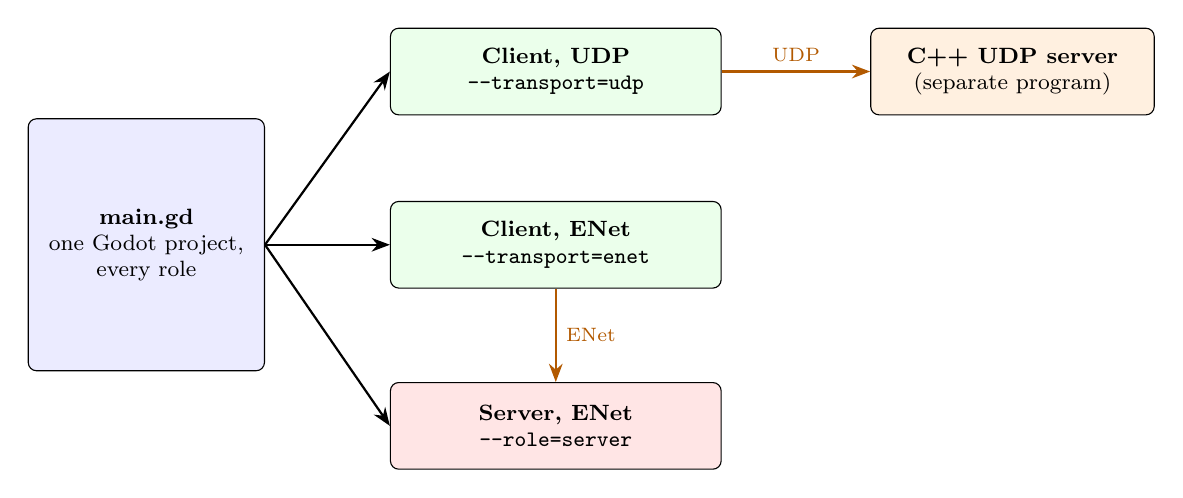
\begin{tikzpicture}[x=1cm,y=1cm,font=\footnotesize,
  box/.style={draw,rounded corners=3pt,align=center,inner sep=5pt,minimum height=1.1cm},
  arr/.style={-{Stealth},thick}]
\node[box,fill=blue!8,minimum width=3.0cm,minimum height=3.2cm] (main) at (0,0) {\textbf{main.gd}\\ one Godot project,\\ every role};
\node[box,fill=green!8,minimum width=4.2cm] (m1) at (5.2,2.2) {\textbf{Client, UDP}\\ \texttt{--transport=udp}};
\node[box,fill=green!8,minimum width=4.2cm] (m2) at (5.2,0) {\textbf{Client, ENet}\\ \texttt{--transport=enet}};
\node[box,fill=red!10,minimum width=4.2cm] (m3) at (5.2,-2.3) {\textbf{Server, ENet}\\ \texttt{--role=server}};
\node[box,fill=orange!12,minimum width=3.6cm] (cpp) at (11,2.2) {\textbf{C++ UDP server}\\ (separate program)};
\foreach \m in {m1,m2,m3} {\draw[arr] (main.east) -- (\m.west);}
\draw[arr,orange!70!black] (m1.east) -- (cpp.west) node[midway,above,font=\scriptsize] {UDP};
\draw[arr,orange!70!black] (m2.south) -- (m3.north) node[midway,right,font=\scriptsize] {ENet};
\end{tikzpicture}
\caption{The Godot project. One script is started in different modes. A UDP client talks to the separate C++ server; an ENet client talks to the same project started as an ENet server.}
\end{figure}

\definecolor{nsbg}{RGB}{72,72,72}
\definecolor{nsgrid}{RGB}{56,56,56}
\definecolor{nspink}{RGB}{235,60,150}
\definecolor{nsyellow}{RGB}{235,212,59}
\definecolor{nscyan}{RGB}{59,205,235}
\newcommand{\nsboard}[1]{% #1 = status text
  \fill[nsbg,rounded corners=2pt] (-0.3,1.0) rectangle (9.1,-9.1);
  \node[white,font=\scriptsize,anchor=west] at (-0.1,0.6) {NodeStrike (DEBUG)};
  \node[white,font=\scriptsize,anchor=east] at (8.9,0.6) {#1};
  \draw[nsgrid,line width=0.3pt] (0,0) grid[step=0.44] (8.8,-8.8);
}
\newcommand{\nsplayer}[4]{% col,row,color,label : filled square
  \fill[#3] ({#1*0.44+0.07},{-#2*0.44-0.07}) rectangle ({#1*0.44+0.37},{-#2*0.44-0.37});
  \node[white,font=\tiny,anchor=south west,inner sep=0.2pt] at ({#1*0.44+0.05},{-#2*0.44-0.38}) {#4};
}
\newcommand{\nsgoal}[3]{% col,row,color : hollow square
  \draw[#3,line width=0.8pt] ({#1*0.44+0.07},{-#2*0.44-0.07}) rectangle ({#1*0.44+0.37},{-#2*0.44-0.37});
}
\newcommand{\nsme}[4]{% col,row,color,label : my square with white outline
  \fill[#3] ({#1*0.44+0.07},{-#2*0.44-0.07}) rectangle ({#1*0.44+0.37},{-#2*0.44-0.37});
  \draw[white,line width=0.9pt] ({#1*0.44+0.07},{-#2*0.44-0.07}) rectangle ({#1*0.44+0.37},{-#2*0.44-0.37});
  \node[white,font=\tiny,anchor=south west,inner sep=0.2pt] at ({#1*0.44+0.05},{-#2*0.44-0.38}) {#4};
}

\begin{figure}[!htbp]
\centering
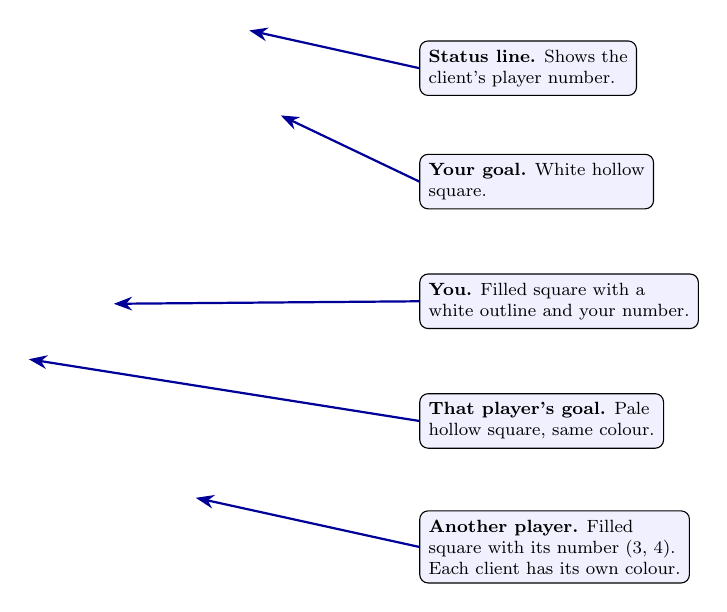
\begin{tikzpicture}[scale=0.8,transform shape,font=\footnotesize,
  note/.style={draw,rounded corners=3pt,fill=blue!6,align=left,inner sep=4pt},
  arr/.style={-{Stealth},thick,blue!60!black}]
\begin{scope}
\nsboard{Connected --- Player \#5}
% other players and their goals
\nsplayer{15}{15}{nsyellow}{3}
\nsgoal{9}{10}{nsyellow!60!white}
\nsplayer{11}{18}{nscyan}{4}
\nsgoal{9}{19}{nscyan!60!white}
% me
\nsgoal{18}{1}{white}
\nsme{12}{8}{nspink}{5}
\end{scope}
\node[note,anchor=west] (a) at (10.6,0.0) {\textbf{Status line.} Shows the\\ client's player number.};
\node[note,anchor=west] (b) at (10.6,-1.8) {\textbf{Your goal.} White hollow\\ square.};
\node[note,anchor=west] (c) at (10.6,-3.7) {\textbf{You.} Filled square with a\\ white outline and your number.};
\node[note,anchor=west] (e) at (10.6,-5.6) {\textbf{That player's goal.} Pale\\ hollow square, same colour.};
\node[note,anchor=west] (d) at (10.6,-7.6) {\textbf{Another player.} Filled\\ square with its number (3, 4).\\ Each client has its own colour.};
\draw[arr] (a.west) -- (7.9,0.6);
\draw[arr] (b.west) -- (8.4,-0.75);
\draw[arr] (c.west) -- (5.75,-3.74);
\draw[arr] (e.west) -- (4.4,-4.62);
\draw[arr] (d.west) -- (7.05,-6.82);
\end{tikzpicture}
\caption{The running NodeStrike client (redrawn from a screenshot of a client started in a window; headless benchmark clients draw nothing). Each tick every bot moves one tile toward its goal. The server's snapshot tells each client where every other player is; the client only draws it. Each player's pale hollow square is that player's goal.}
\end{figure}

\newcommand{\nsmini}{% small board, no header
  \fill[nsbg,rounded corners=1pt] (-0.1,0.1) rectangle (4.5,-4.5);
  \draw[nsgrid,line width=0.2pt] (0,0) grid[step=0.22] (4.4,-4.4);
}
\newcommand{\nsminisq}[3]{% col,row,color
  \fill[#3] ({#1*0.22+0.03},{-#2*0.22-0.03}) rectangle ({#1*0.22+0.19},{-#2*0.22-0.19});
}
\newcommand{\nsminigoal}[3]{%
  \draw[#3,line width=0.5pt] ({#1*0.22+0.03},{-#2*0.22-0.03}) rectangle ({#1*0.22+0.19},{-#2*0.22-0.19});
}
\newcommand{\nsminime}[3]{%
  \fill[#3] ({#1*0.22+0.03},{-#2*0.22-0.03}) rectangle ({#1*0.22+0.19},{-#2*0.22-0.19});
  \draw[white,line width=0.6pt] ({#1*0.22+0.03},{-#2*0.22-0.03}) rectangle ({#1*0.22+0.19},{-#2*0.22-0.19});
}
\newcommand{\nsworld}[1]{% the three players; #1 = code to draw "me" outline or plain
  \nsminisq{15}{15}{nsyellow}\nsminigoal{9}{10}{nsyellow!60!white}
  \nsminisq{11}{18}{nscyan}\nsminigoal{9}{19}{nscyan!60!white}
  \nsminigoal{18}{1}{#1}
}
\newcommand{\nstable}[1]{%
  \begin{tabular}{@{}rrrrr@{}}
  \textbf{id} & \textbf{x} & \textbf{y} & \textbf{gx} & \textbf{gy}\\
  \textcolor{nsyellow!70!black}{3} & 15 & 15 & 9 & 10\\
  \textcolor{nscyan!70!black}{4} & 11 & 18 & 9 & 19\\
  \textcolor{nspink}{5} & 12 & 8 & 18 & 1\\
  \end{tabular}}

\begin{figure}[!htbp]
\centering
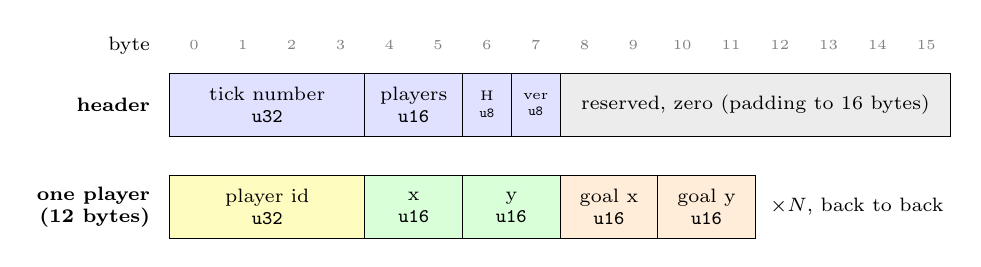
\begin{tikzpicture}[x=0.62cm,y=1cm,font=\footnotesize,
  cell/.style={draw,minimum height=0.8cm,inner sep=0pt,align=center,font=\scriptsize}]
\foreach \i in {0,...,15} {\node[font=\tiny,gray] at (\i+0.5,0.35) {\i};}
\node[font=\scriptsize,anchor=east] at (-0.2,0.35) {byte};
\node[font=\scriptsize\bfseries,anchor=east] at (-0.2,-0.4) {header};
\node[cell,fill=blue!12,minimum width=2.48cm] at (2,-0.4) {tick number\\\texttt{u32}};
\node[cell,fill=blue!12,minimum width=1.24cm] at (5,-0.4) {players\\\texttt{u16}};
\node[cell,fill=blue!12,minimum width=0.62cm,font=\tiny] at (6.5,-0.4) {H\\\texttt{u8}};
\node[cell,fill=blue!12,minimum width=0.62cm,font=\tiny] at (7.5,-0.4) {ver\\\texttt{u8}};
\node[cell,fill=gray!15,minimum width=4.96cm] at (12,-0.4) {reserved, zero (padding to 16 bytes)};
\node[font=\scriptsize\bfseries,anchor=east,align=right] at (-0.2,-1.7) {one player\\(12 bytes)};
\node[cell,fill=yellow!25,minimum width=2.48cm] at (2,-1.7) {player id\\\texttt{u32}};
\node[cell,fill=green!15,minimum width=1.24cm] at (5,-1.7) {x\\\texttt{u16}};
\node[cell,fill=green!15,minimum width=1.24cm] at (7,-1.7) {y\\\texttt{u16}};
\node[cell,fill=orange!15,minimum width=1.24cm] at (9,-1.7) {goal x\\\texttt{u16}};
\node[cell,fill=orange!15,minimum width=1.24cm] at (11,-1.7) {goal y\\\texttt{u16}};
\node[font=\scriptsize,anchor=west] at (12.1,-1.7) {$\times N$, back to back};
\end{tikzpicture}
\caption{Layout of one snapshot, $16 + 12N$ bytes (52 bytes for 3 players, 3\,616 for 300). The ENet server writes it into one byte array and sends it as a remote procedure call; the C++ server sends the same bytes directly in UDP datagrams of at most 1\,200 bytes.}
\label{fig:snapshot}
\end{figure}


\subsection{C++ UDP server}
% [PROPOSAL] Sources: "What is being built from scratch", "Packet Format", "Heartbeat and Client Eviction".
%   - Planned design (matches the code): single-threaded receive loop, client registry keyed by IP and port, fixed-tick state
%     broadcast, heartbeat eviction, binary packet format. -> reuse as the goals paragraph ("design decisions").
%   - Packet format. The proposal: one-byte message ID then a payload; messages CONNECT, INPUT (movement vector + sequence number),
%     STATE (positions), HEARTBEAT (once per second) and DISCONNECT. [CHECK] The built protocol (Table~\ref{tab:packets}) is
%     version 2 with JOIN, ACK, STATE and TICK only: no separate INPUT, HEARTBEAT or DISCONNECT. Say that the design changed and
%     why (e.g. the STATE message sent every tick already works as a heartbeat; there is no explicit disconnect, silent clients
%     time out). Make sure that is actually how the code behaves before writing it.
%   - Heartbeat and eviction: the proposal says the 5 s timeout was chosen to match the ENet server's default, so connection
%     management is comparable. -> reuse this reasoning; it explains the "Client eviction" row of Table~\ref{tab:compare}.
%     [CHECK] The proposal says the server compares the clock with every client's last-seen time on each loop pass, but the
%     notes below say the check happens once per tick; describe the code, not the proposal.
%   - "Problems you hit" (asked for in the TODO) already exists in this file: the tick drift (Section~\ref{sec:fixes}). Summarize
%     it here in two sentences and point there.
% TODO: write how the C++ server was built (goals, design decisions, problems you hit) (see next line)
TODO: write how the C++ server was built (goals, design decisions, problems you hit).
%TODO write how the C++ server was built (goals, design decisions, problems you hit

% \paragraph{Notes from the code (delete when written).}
% \begin{itemize}
% \item One file, \texttt{server/main.cpp} (about 590 lines), C++17, plain POSIX sockets, one thread.
% \item Binary protocol, version 2 (Table~\ref{tab:packets}). A player is identified by its network address, not by anything the client sends.
% \item Main loop (Figure~\ref{fig:cppLoop}): wait for a packet (until the next tick is due, at most 5~ms), read everything waiting, and when the next tick is due, run it.
% \item A tick drops clients silent for more than 5~s and sends a snapshot to every client, split into datagrams of at most 1,200 bytes.
% \item Once a second it prints one telemetry line (tick number, players, packets and bytes in and out); the benchmark records these lines.
% \item A separate terminal display, \texttt{tui/tui.cpp}, exists for watching a server.
% \end{itemize}

\begin{table}[H]
\centering
\small
\begin{tabular}{@{}llrl@{}}
\toprule
Message & Direction & Size & Contents \\
\midrule
JOIN & client to server & 2 B & type, version \\
ACK & server to client & 6 B & type, version, player id \\
STATE & client to server & 18 B & position, timestamp, number, goal \\
TICK (snapshot) & server to client & 16 + 12N B & header, then id, position and goal for each of N players \\
\bottomrule
\end{tabular}
\caption{Messages of the C++ server protocol (version 2). Snapshots larger than 1,200 bytes are split into several datagrams.}
\label{tab:packets}
\end{table}

\subsection{The two backends compared}
% [PROPOSAL] Reuse the proposal's "Headless Mode and Engine Overhead" argument here as the reason the two servers differ:
%   in a normal Godot client the engine runs rendering, audio, physics, game logic and networking; the dedicated-server export
%   drops rendering and audio but keeps physics, game logic and networking inside the engine process; the C++ server runs
%   only networking and the minimum game logic. The proposal says this difference "is precisely what the benchmark is designed
%   to characterize".
% [CHECK] Do not claim the overhead is the cause of any measured difference unless you measured it (e.g. profiled the Godot
%   process). What you can say is that ENet's server used more CPU (compare the CPU columns in Tables~\ref{tab:ladder} and
%   \ref{tab:holdsum}) and the proposal's explanation is a candidate. Keep that wording for the Discussion too.
% [CHECK] Table~\ref{tab:compare} is the main content of this section; the text should walk through its rows (networking, tick
%   timing, join, position update, snapshot, eviction, latency measure, telemetry) and say which differences are intended and
%   which were removed to keep the test fair (header size, tick schedule).
% TODO: write how the two servers work and how they differ (see next line)
TODO: write how the two servers work and how they differ.

\begin{table}[H]
\centering
\small
\begin{tabular}{@{}p{0.2\textwidth}p{0.36\textwidth}p{0.36\textwidth}@{}}
\toprule
& C++ UDP server & Godot ENet server \\
\midrule
Networking & raw UDP datagrams & ENet through Godot's multiplayer peer \\
Default port & 7777 & 7778 \\
Tick timing & fixed-timestep schedule: each tick is due at an exact multiple of 50 ms, so it runs at 20 ticks per second (the first version restarted its timer at each tick and drifted to about 19, see Section~\ref{sec:fixes}) & Godot timer that fires every 50 ms and keeps its timetable (20 ticks per second) \\
Join & JOIN message, ACK with player id & connection handled by ENet; the peer id is the player id \\
Position update & 18-byte STATE datagram (position, timestamp, number, goal), sent every tick & \texttt{submit\_state} remote procedure call (unreliable) with the same fields, sent every tick \\
Snapshot & 16 + 12N bytes, split into datagrams of at most 1,200 B & 16 + 12N bytes (binary format, header padded from 8 to 16 bytes so both sizes match), one remote procedure call \\
Client eviction & silent for 5 s & silent for 5 s \\
Latency measure & game client's ping: last send until next snapshot & same Godot client script, same measure \\
Telemetry & one line per second & periodic server statistics \\
\bottomrule
\end{tabular}
\caption{The two backends side by side.}
\label{tab:compare}
\end{table}

\section{Methodology}\label{sec:data}
% [PROPOSAL] Sources: "Experiment Design" (6.1 Procedure, 6.2 Variable and control, 6.3 Data Analysis and Measurement) and
%   "Primary Objective". The structure carries over, but most of the setup changed. What changed:
%
%   Proposal                                          | This paper
%   --------------------------------------------------|------------------------------------------------------------
%   Client counts 1, 5, 10, 20, 50 (H1: 30 to 50)     | Ladder 1, 10..300 (292 states); holds at 180/260/270/300
%   3 repetitions, 8 min per step                     | 8 runs per backend; 10 s per ladder state; 20 min holds
%   Both backends on the same host machine            | Google Cloud: 1 server VM + 3 client VMs (private network)
%   Headless Godot clients in containers              | Headless Godot bot clients on 3 VMs (script-controlled)
%   Wireshark on the host interface + per-packet      | Per-second server telemetry + per-state client counters
%     client CSV timestamps                           |   + per-second CPU/memory/network on every VM
%   Latency = end-to-end round trip (ms)              | Ping proxy: last send until next snapshot (includes tick wait)
%   Throughput = packets/s from Wireshark; bandwidth  | Snapshots received per client per second; server packet/byte
%     MB/s from capture stats                         |   counters exist in telemetry but bandwidth is not reported
%   Packet loss = (sent - received) / sent            | Snapshot sequence-number gaps ("protocol-level loss")
%   Capacity = highest count without degradation      | Clients responding + health limits (see Health criteria)
%   Significance testing (H0/H1, Task 1.5)            | Currently only mean and lowest/highest run (see [CHECK] below)
%
%   Reusable from the proposal: the independent variables (backend, number of clients), the idea of restarting the backend
%   between windows, and the list of controlled variables. [CHECK] The proposal's controls include the host machine, network
%   interface, kernel socket-buffer parameters, Godot client build, NodeStrike logic/tick rate and time of day. Say which of those
%   are still controlled (same zone, same VM types, same client script and 20 Hz) and which are not (kernel buffer settings,
%   time of day) so a reader knows what is held constant.
% [CHECK] The proposal promised a test for statistically significant differences (Task 1.5, and the H0/H1 pair). The paper
%   so far reports means with lowest/highest run only. Either add a test (8 runs per backend, e.g. Mann-Whitney U on per-run
%   gap counts) or state clearly that the analysis is descriptive and why. The Discussion and Conclusion depend on which.
% [CHECK] The proposal says server and clients share one machine; here they are on separate VMs. Network latency between VMs is
%   therefore part of every ping number. Say that in the text so readers do not compare the ping values with local-host numbers.

All runs use one server VM and three client VMs on Google Cloud (the server on an e2-standard-2 machine, the clients on n2-standard-4 machines).
ENet snapshots use the binary format from 22 September onward.

\subsection{Main measures}
Three measures are the main focus of the study. The rest of the data (CPU, memory,
network use, server counters and every other column collected) is kept and still matters:
it is used to explain why the main measures change. A tick-rate drop is the warning sign
that one of the three is failing.

\begin{table}[H]
\centering
\small
\begin{tabular}{@{}p{0.2\textwidth}p{0.36\textwidth}p{0.31\textwidth}@{}}
\toprule
Measure & Plain meaning & On the charts \\
\midrule
Latency & How long data takes to go to the server and back, in milliseconds (ping). Lower is better. & Ping in milliseconds (log scale) \\
Packet handling & How many packets the server receives and sends each second without losing or delaying them. A healthy client gets one snapshot per tick, about 20 per second. & Snapshots received per client per second (20 is perfect) \\
Client limit & The largest number of clients the server supports before performance degrades. & Share of clients still responding; where the lines break \\
Tick rate (warning sign) & Ticks the server completes per second. 20 Hz is healthy; below 18 Hz means the server is falling behind. & Server ticks per second, with an 18~Hz line \\
\bottomrule
\end{tabular}
\caption{The three main measures, and the tick-rate warning sign. All other collected data supports them.}
\end{table}


\subsection{Two kinds of test}
We run two kinds of test, because they answer different questions.

\begin{itemize}
\item \textbf{Progressive (granular) ladder.} Start with one client and add
clients one step at a time, holding each step for a short time (10~s in the
October runs). The state list is 1 client, then 10, 11, 12, up to 300: 292
states per backend. Question: at what client count does the server stop
keeping up?
\item \textbf{Hold.} Ramp up to a target client count (targets 180, 260,
270 and 300), stop adding clients, and keep them connected for 20 minutes,
measured in 120 windows of 10~s. Question: does the server stay stable at a
fixed load?
\end{itemize}

\subsection{How the data is collected}
Figure~\ref{fig:fleet} shows where a test runs. A Python script automates every run:

\begin{enumerate}
\item It creates one server VM and three client VMs on Google Cloud.
\item It starts the server (the C++ UDP server, or the Godot ENet server in headless mode).
\item It gives each client VM a plan: a list of states, each with a
total client target and a duration. The client VMs start bot clients so that the
total matches the plan, and each bot plays the NodeStrike game. Every bot is the same Godot client (\texttt{main.gd}): in UDP mode it talks to the C++ server and in ENet mode to the Godot server, so both servers are driven by the same client code.
\item During every state, each client counts what it sent and received, checks
the snapshot sequence numbers for gaps, and measures ping about once per second.
\item The server writes one telemetry row per second (tick count, players
connected, packets and bytes in and out). Each VM also records CPU, memory and
network use every second.
\item When the run ends, all files are downloaded to the runner, the VMs are
deleted, and analysis scripts merge the repetitions and apply pass/fail
thresholds.
\end{enumerate}

\begin{figure}[!htbp]
\centering
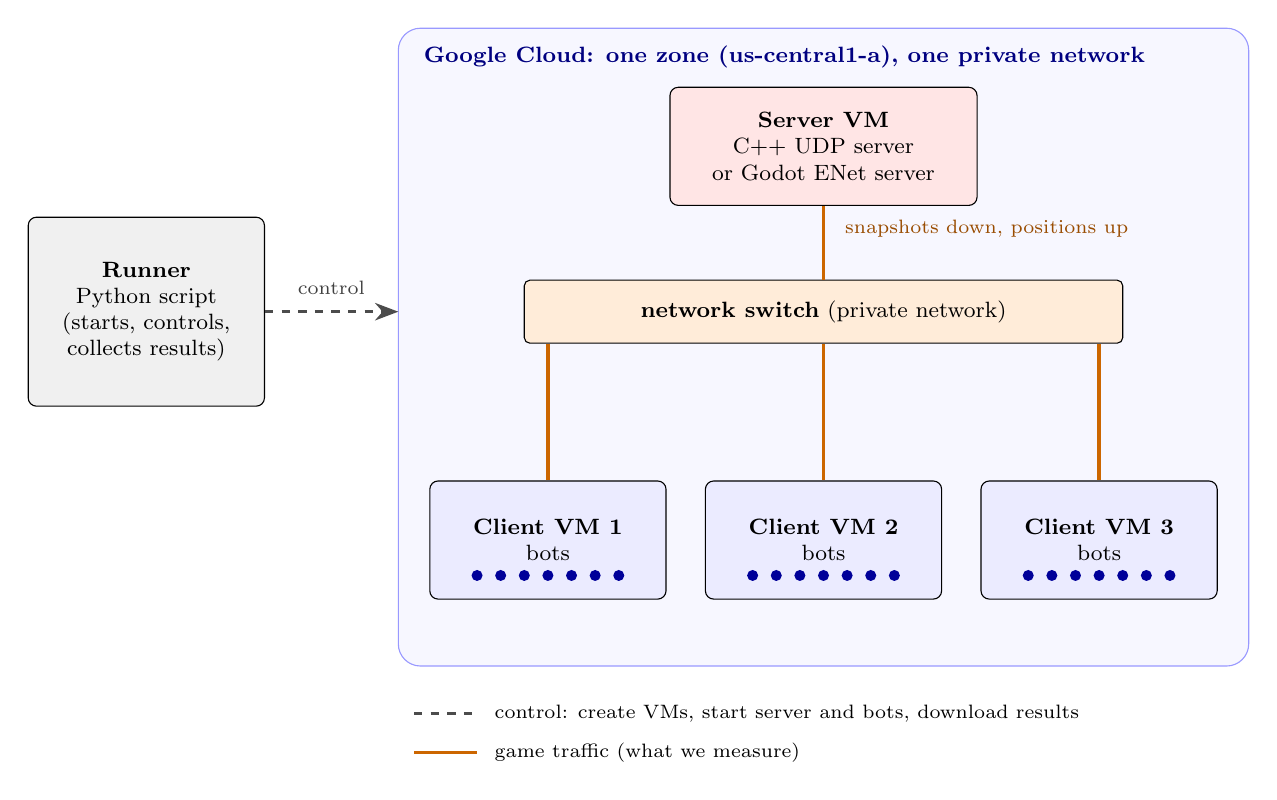
\begin{tikzpicture}[x=1cm,y=1cm,font=\footnotesize,
  vm/.style={draw,rounded corners=3pt,fill=blue!8,minimum width=3.0cm,minimum height=1.5cm,align=center,inner sep=4pt},
  srv/.style={draw,rounded corners=3pt,fill=red!10,minimum width=3.9cm,minimum height=1.5cm,align=center,inner sep=4pt},
  net/.style={orange!80!black,very thick}]
% cloud
\draw[rounded corners=8pt,fill=blue!3,draw=blue!40] (4.7,-4.6) rectangle (15.5,3.5);
\node[anchor=north west,font=\bfseries\footnotesize,text=blue!50!black] at (4.9,3.4) {Google Cloud: one zone (us-central1-a), one private network};
% runner
\node[draw,rounded corners=3pt,fill=gray!12,minimum width=3.0cm,minimum height=2.4cm,align=center] (run) at (1.5,-0.1) {\textbf{Runner}\\ Python script\\ (starts, controls,\\ collects results)};
\draw[gray!60!black,dashed,very thick,-{Stealth}] (run.east) -- (4.7,-0.1);
\node[font=\scriptsize,gray!50!black,align=center,anchor=south] at (3.85,0.0) {control};
% switch
\node[draw,rounded corners=2pt,fill=orange!15,minimum width=7.6cm,minimum height=0.8cm,align=center] (sw) at (10.1,-0.1) {\textbf{network switch} (private network)};
% server
\node[srv] (srv) at (10.1,2.0) {\textbf{Server VM}\\ C++ UDP server\\ or Godot ENet server};
% clients
\node[vm] (c1) at (6.6,-3.0) {\textbf{Client VM 1}\\ bots};
\node[vm] (c2) at (10.1,-3.0) {\textbf{Client VM 2}\\ bots};
\node[vm] (c3) at (13.6,-3.0) {\textbf{Client VM 3}\\ bots};
\foreach \x in {6.6,10.1,13.6} {\foreach \d in {-0.9,-0.6,...,0.9} {\fill[blue!60!black] (\x+\d,-3.45) circle (0.07);}}
% game traffic
\draw[net] (srv.south) -- (srv.south |- sw.north);
\foreach \c in {c1,c2,c3} {\draw[net] (\c.north) -- (\c.north |- sw.south);}
\node[font=\scriptsize,orange!60!black,anchor=west] at (10.25,0.95) {snapshots down, positions up};
% legend
\draw[gray!60!black,dashed,very thick] (4.9,-5.2) -- (5.7,-5.2);
\node[anchor=west,font=\scriptsize] at (5.8,-5.2) {control: create VMs, start server and bots, download results};
\draw[net] (4.9,-5.7) -- (5.7,-5.7);
\node[anchor=west,font=\scriptsize] at (5.8,-5.7) {game traffic (what we measure)};
\end{tikzpicture}
\caption{Where a test runs. The runner creates one server VM and
three client VMs, starts the server, tells each client VM how many bots to run,
and downloads the results afterwards. The bots and the server talk to each other
over the cloud's private network (a switch). Each client VM runs about a third of
the bots, so the server sees all of them as one crowd.}
\label{fig:fleet}
\end{figure}

Gaps and incomplete snapshots are indicators of protocol-level loss, not
measured network packet-loss percentages.


\subsection{Health criteria and caveats}
% [PROPOSAL] The proposal defines capacity only as "the highest client count sustained without measurable degradation", with no
%   numbers. The numeric limits now exist but are only written in the caption of Table~\ref{tab:holdsum}: at least 99\% of
%   clients responding, at least 18 snapshots per second per client, ping at most 150 ms, server tick at least 18 Hz. Put them
%   here as a list or small table, and say how a ladder state "passes" (Table~\ref{tab:limit}) versus how a hold "holds".
% [NEW] Caveats to write (these are in the paper's text already, scattered; collect them here):
%   - ping is a proxy: it includes waiting for the next 50 ms tick, so it is not a true round trip (the proposal wording
%     "end-to-end round-trip latency" must not be reused);
%   - gaps are protocol-level losses, not measured network packet-loss percentages;
%   - one cloud zone, one server machine type, bot clients rather than real players, one workload;
%   - the last ladder state artifact and the slow-state timing quirk (Section~\ref{sec:fixes}).
% TODO: write the pass/fail limits and what the measurements can and cannot show (see next line)
TODO: write the pass/fail limits and what the measurements can and cannot show.

\subsection{Precision limits}
\label{sec:precision}
% TODO: write the precision limit for each quantity and name the limiting proposition (verify the granularities below)
TODO: write the precision limits.

\begin{table}[H]
\centering
\footnotesize
\begin{tabular}{@{}llp{6.2cm}@{}}
\toprule
Quantity & Granularity & Where the limit comes from \\
\midrule
Ping proxy & 1~ms & The client logs whole milliseconds, but a snapshot only arrives every 50~ms (20~Hz), so differences of a few ms between backends are not reliable (limiting quantity). \\
Server tick rate & 0.01~Hz & Computed from 9--10 samples in each 10~s window. \\
Snapshots per client per second & 0.01 & Count over a 10~s window divided by the clients. \\
Packet gaps & 1 snapshot & Integer count of skipped snapshot numbers. \\
Clients responding & 1 client & Whole clients. \\
CPU & 0.1~\% & Sampled once per second and averaged over the window. \\
\bottomrule
\end{tabular}
\caption{Granularity of each measured quantity. The precision limit of a conclusion is set by the coarsest quantity it relies on.}
\label{tab:precision}
\end{table}

\subsection{Runs}

Granular ramps with $N_{\max}=300$ give 292 states per backend
($1$ plus $10$ through $300$).

\begin{table}[H]
\centering
\footnotesize
\setlength{\tabcolsep}{3pt}
\begin{tabular}{@{}llllrrl@{}}
\toprule
Date (2026) & Type & Backend & Counts & Time/state & Runs & Status \\
\midrule
Oct 23--24 & Progressive ladder (granular) & C++ server, ENet server & 1, 10--300 & 10~s & 8 runs & ok \\
Oct 24 & Hold & C++ server, ENet server & 180, 260, 270, 300 & 20~min hold & 8 runs & ok \\
\bottomrule
\end{tabular}
\caption{Runs used in the results. The progressive ladder is eight complete runs per backend, each run a separate pass from 1 to 300 clients (one repetition each). The C++ server is driven by Godot UDP clients and the ENet server by Godot ENet clients. The hold tests are eight runs per backend and target, each a 20-minute hold (one repetition each) after a ramp-up of 10 clients per 10~s.}
\end{table}

\subsection{How the runs were summed up}
Both tests combine 8 complete runs per backend. For the ladder, each of the 292 client counts is paired with the same count in the other runs. For the holds, each 10~s state is paired by its position in the ramp-up or hold. The mean, lowest and highest value of each measure are reported. A ladder run passes at a client count if that count met the health limits; a hold run held if its hold averages met them. Hold run 5 needed a second attempt; its first attempt is not used.

\subsection{Implementation validation}\label{sec:fixes}
% TODO: rewrite this subsection in your own words. Everything below is taken from the old Section 7 (which stays in main.tex).
\begin{table}[H]
\centering
\footnotesize
\setlength{\tabcolsep}{3pt}
\begin{tabular}{p{0.25\columnwidth}p{0.26\columnwidth}p{0.25\columnwidth}p{0.12\columnwidth}}
\toprule
Problem & Why it mattered & Fix & Status \\
\midrule
C++ ticks drifted to about 19~Hz & C++ did about 5\% fewer ticks per second than ENet & Fixed-timestep tick schedule & Fixed \\
Snapshot sizes differed (8 vs 16 header bytes) & ENet sent slightly smaller packets than C++ & ENet header padded to 16 bytes & Fixed \\
Slow ENet states and a last-state artifact & ENet rates were measured over longer windows; the last ladder state was inflated & To be handled in the analysis & Noted \\
\bottomrule
\end{tabular}
\caption{Problems found in the first runs.}
\label{tab:problems}
\end{table}

Two changes were made in \texttt{server/main.cpp}. First, the next tick is scheduled at an exact multiple of 50~ms after the previous due time, so lateness does not add up. Second, the wait for packets now ends when the next tick is due (at most 5~ms), so ticks are noticed sooner. If the server ever falls more than a whole tick behind, it resynchronizes instead of firing a burst of ticks. Figure~\ref{lst:fixed} shows the code. In a 30-second local test the original server ticked at 19.67~Hz and the fixed server at 20.000~Hz.

\begin{figure}[H]
\begin{lstlisting}[language=C++]
const auto tick_period = std::chrono::duration_cast<Clock::duration>(
                             std::chrono::duration<double>(TICK_SEC));
auto next_tick = Clock::now() + tick_period;
while (true) {
    // ... wait for packets until next_tick (at most 5 ms) ...
    auto now = Clock::now();
    if (now >= next_tick) {
        next_tick += tick_period;
        if (next_tick <= now)    // a whole tick behind: resync
            next_tick = now + tick_period;
        // ... tick: drop silent clients, broadcast snapshots ...
    }
}
\end{lstlisting}
\caption{The fixed-timestep tick schedule in the C++ server (excerpt from \texttt{server/main.cpp}). The key change is \texttt{next\_tick += tick\_period}: the next tick is due one period after the previous due time, not after the moment the tick was noticed.}
\label{lst:fixed}
\end{figure}

\begin{itemize}
\item \textbf{Slow ENet states.} When ENet was overloaded, a ``10~s'' ladder state actually lasted about 27~s, because the harness waited for slow client logs. Rates are computed over the real length, so they are correct.
\item \textbf{The last ladder state.} The last state (300 clients) has no later state to measure its length from, so the nominal 10~s was used while its counters covered about 27~s. This inflated its snapshot rate (up to about 30 per second, which cannot be real at 20 ticks per second).
\end{itemize}
The last ladder state is left out of the corrected ladder plots and tables (Section~\ref{sec:ladder}).

\section{Results}\label{sec:results}
% [PROPOSAL] The proposal has no results. Its analysis plan (6.3) was: latency distribution per backend, packets per second,
%   loss from sent versus received counts, bandwidth from Wireshark. Only the first two have a counterpart here; see the
%   comparison table at the top of Experimental Method.

\subsection{Test 1, progressive ladder: granular runs (both patches applied)}
\label{sec:ladder}
% [NEW] Things the tables already show (check them against the CSVs before you write them as findings):
%   - C++ server: gaps are 0 at every selected count (run 8 had 5 gaps in total); 291--292 of 292 states passed in every run.
%   - ENet server: gaps first appear around 150--200 clients (Table~\ref{tab:ladder}: 0 at 100, 10 at 200, 38 at 250, 116 at 300)
%     and total 3,900--7,000 per run (Table~\ref{tab:limit}); ping and tick rate are close to C++ (tick about 20 Hz for both).
%   - So "client limit" is not a single sharp number for either server in this data: all states mostly pass. Decide how to
%     define it (e.g. first count with sustained gaps, or first failing state per run, 294 in ENet run 3) before writing.
TODO: interpret the ladder results (latency, packet gaps, client limit, tick rate).

\begin{figure}[!htbp]
\centering
{\bfseries\small Test 1: progressive ladder, 10 to 299 clients (mean of 8 runs, 10~s per client count)\par}\vspace{4pt}
\begin{tikzpicture}
\begin{groupplot}[group style={group size=2 by 2,horizontal sep=1.7cm,vertical sep=1.9cm},
  width=0.5\textwidth,height=4.1cm,xlabel={clients},xmin=10,xmax=299,
  tick label style={font=\scriptsize},label style={font=\footnotesize},
  title style={font=\footnotesize\bfseries},grid=major,grid style={gray!25}]
\nextgroupplot[title={Latency (ping proxy)},ylabel={ms},ymin=0]
\addplot[name path=picp0lo,draw=none,forget plot] table[x=nclients,y=ping_min,col sep=comma]{data/g8_cppgodot.csv};
\addplot[name path=picp0hi,draw=none,forget plot] table[x=nclients,y=ping_max,col sep=comma]{data/g8_cppgodot.csv};
\addplot[blue!70!black!25,forget plot] fill between[of=picp0lo and picp0hi];
\addplot[blue!70!black,thick,mark=none] table[x=nclients,y=ping_mean,col sep=comma]{data/g8_cppgodot.csv};
\addplot[name path=pien0lo,draw=none,forget plot] table[x=nclients,y=ping_min,col sep=comma]{data/g8_enet.csv};
\addplot[name path=pien0hi,draw=none,forget plot] table[x=nclients,y=ping_max,col sep=comma]{data/g8_enet.csv};
\addplot[red!70!black!25,forget plot] fill between[of=pien0lo and pien0hi];
\addplot[red!70!black,thick,mark=none] table[x=nclients,y=ping_mean,col sep=comma]{data/g8_enet.csv};
\nextgroupplot[title={Packet gaps},ylabel={missed snapshots per state},ymin=0]
\addplot[name path=gacp1lo,draw=none,forget plot] table[x=nclients,y=gaps_min,col sep=comma]{data/g8_cppgodot.csv};
\addplot[name path=gacp1hi,draw=none,forget plot] table[x=nclients,y=gaps_max,col sep=comma]{data/g8_cppgodot.csv};
\addplot[blue!70!black!25,forget plot] fill between[of=gacp1lo and gacp1hi];
\addplot[blue!70!black,thick,mark=none] table[x=nclients,y=gaps_mean,col sep=comma]{data/g8_cppgodot.csv};
\addplot[name path=gaen1lo,draw=none,forget plot] table[x=nclients,y=gaps_min,col sep=comma]{data/g8_enet.csv};
\addplot[name path=gaen1hi,draw=none,forget plot] table[x=nclients,y=gaps_max,col sep=comma]{data/g8_enet.csv};
\addplot[red!70!black!25,forget plot] fill between[of=gaen1lo and gaen1hi];
\addplot[red!70!black,thick,mark=none] table[x=nclients,y=gaps_mean,col sep=comma]{data/g8_enet.csv};
\nextgroupplot[title={Packet handling},ylabel={snapshots/s per client},ymin=0,ymax=26]
\addplot[name path=recp2lo,draw=none,forget plot] table[x=nclients,y=recv_min,col sep=comma]{data/g8_cppgodot.csv};
\addplot[name path=recp2hi,draw=none,forget plot] table[x=nclients,y=recv_max,col sep=comma]{data/g8_cppgodot.csv};
\addplot[blue!70!black!25,forget plot] fill between[of=recp2lo and recp2hi];
\addplot[blue!70!black,thick,mark=none] table[x=nclients,y=recv_mean,col sep=comma]{data/g8_cppgodot.csv};
\addplot[name path=reen2lo,draw=none,forget plot] table[x=nclients,y=recv_min,col sep=comma]{data/g8_enet.csv};
\addplot[name path=reen2hi,draw=none,forget plot] table[x=nclients,y=recv_max,col sep=comma]{data/g8_enet.csv};
\addplot[red!70!black!25,forget plot] fill between[of=reen2lo and reen2hi];
\addplot[red!70!black,thick,mark=none] table[x=nclients,y=recv_mean,col sep=comma]{data/g8_enet.csv};
\draw[dashed,gray] (axis cs:10,20) -- (axis cs:299,20);
\nextgroupplot[title={Server CPU},ylabel={\% of one VM},ymin=0]
\addplot[name path=sccp5lo,draw=none,forget plot] table[x=nclients,y=scpu_min,col sep=comma]{data/g8_cppgodot.csv};
\addplot[name path=sccp5hi,draw=none,forget plot] table[x=nclients,y=scpu_max,col sep=comma]{data/g8_cppgodot.csv};
\addplot[blue!70!black!25,forget plot] fill between[of=sccp5lo and sccp5hi];
\addplot[blue!70!black,thick,mark=none] table[x=nclients,y=scpu_mean,col sep=comma]{data/g8_cppgodot.csv};
\addplot[name path=scen5lo,draw=none,forget plot] table[x=nclients,y=scpu_min,col sep=comma]{data/g8_enet.csv};
\addplot[name path=scen5hi,draw=none,forget plot] table[x=nclients,y=scpu_max,col sep=comma]{data/g8_enet.csv};
\addplot[red!70!black!25,forget plot] fill between[of=scen5lo and scen5hi];
\addplot[red!70!black,thick,mark=none] table[x=nclients,y=scpu_mean,col sep=comma]{data/g8_enet.csv};
\end{groupplot}
\node[anchor=north] at ($(group c1r2.south east)!0.5!(group c2r2.south west)+(0,-1.5cm)$) {\footnotesize \textcolor{blue!70!black}{\rule[0.5ex]{1.2em}{1.2pt}} C++ server \quad \textcolor{red!70!black}{\rule[0.5ex]{1.2em}{1.2pt}} ENet server \quad shaded band: lowest to highest run};
\end{tikzpicture}
\caption{Test 1, progressive ladder (granular batch, both patches applied; server on an e2-standard-2 VM, three n2-standard-4 client VMs, 10~s per client count; the 1-client warm-up state and the last state, 300 clients, are left out: the last state has no later state to time it by, so its counters cover a longer period than 10~s, see Section~\ref{sec:fixes}). Each line is the mean of 8 runs and the band spans the lowest to the highest run. The C++ server is driven by Godot UDP clients and the ENet server by Godot ENet clients. Ping is measured by the Godot client (time from its last send until a snapshot arrives), not a true round trip. Packet gaps are skipped snapshot numbers summed over all clients in a state. Dashed lines: 20 snapshots per second and the 18~Hz tick threshold. Clients responding was 100\% in every state and the server tick rate stayed between 19.9 and 20.1~Hz for both servers (Table~\ref{tab:ladder}), so those two panels are left out.}
\label{fig:ladder}
\end{figure}

\begin{table}[H]
\centering
\small
\setlength{\tabcolsep}{3pt}
\begin{tabular}{@{}lrrrrrrr@{}}
\toprule
Backend & Clients & Resp. (\%) & Ping, ms & Snap/s & Gaps & Tick (Hz) & Srv CPU (\%) \\
\midrule
C++ server & 100 & 100.0 & 29 (26--31) & 19.9 (19.9--20.0) & 0 (0--0) & 20.00 & 4.4 \\
C++ server & 150 & 100.0 & 30 (29--32) & 19.9 (19.8--19.9) & 0 (0--0) & 20.00 & 6.4 \\
C++ server & 200 & 100.0 & 33 (32--35) & 19.8 (19.7--19.9) & 0 (0--0) & 20.00 & 8.9 \\
C++ server & 250 & 100.0 & 35 (33--37) & 19.6 (19.5--19.9) & 0 (0--0) & 20.00 & 10.2 \\
C++ server & 299 & 100.0 & 39 (38--41) & 19.0 (18.8--19.3) & 0 (0--0) & 20.00 & 13.3 \\
\midrule
ENet server & 100 & 100.0 & 28 (25--30) & 19.9 (19.9--20.0) & 0 (0--0) & 20.01 & 4.7 \\
ENet server & 150 & 100.0 & 30 (28--31) & 19.9 (19.9--19.9) & 0 (0--1) & 20.01 & 7.8 \\
ENet server & 200 & 100.0 & 33 (32--34) & 19.8 (19.8--19.9) & 10 (7--16) & 20.00 & 9.5 \\
ENet server & 250 & 100.0 & 33 (33--34) & 19.7 (19.5--19.8) & 38 (20--85) & 20.00 & 13.5 \\
ENet server & 299 & 100.0 & 37 (36--40) & 18.9 (18.4--19.1) & 145 (116--201) & 19.99 & 16.6 \\
\bottomrule
\end{tabular}
\caption{Ladder results at selected client counts, summed up over 8 runs (10~s per state). Ping, Snap/s and Gaps show the mean and, in brackets, the lowest and highest run. Resp.\ = clients responding (mean); Ping = the Godot client's ping proxy; Snap/s = snapshots received per client per second; Gaps = skipped snapshot numbers in that state; Tick = server ticks per second; Srv CPU = server CPU.}
\label{tab:ladder}
\end{table}

\begin{table}[H]
\centering
\small
\begin{tabular}{@{}rrrrrrr@{}}
\toprule
& \multicolumn{3}{c}{C++ server} & \multicolumn{3}{c}{ENet server} \\
Run & Passed & Gaps & First fail & Passed & Gaps & First fail \\
\midrule
1 & 291 & 0 & -- & 290 & 4{,}257 & -- \\
2 & 291 & 0 & -- & 290 & 3{,}807 & -- \\
3 & 290 & 0 & -- & 287 & 5{,}367 & 294 \\
4 & 290 & 0 & -- & 290 & 6{,}951 & -- \\
5 & 290 & 0 & -- & 291 & 4{,}722 & -- \\
6 & 290 & 0 & -- & 290 & 4{,}267 & -- \\
7 & 291 & 0 & -- & 290 & 5{,}847 & -- \\
8 & 290 & 5 & -- & 291 & 4{,}710 & -- \\
\bottomrule
\end{tabular}
\caption{Per run, over the ladder (291 states, 1 and 10 to 299 clients): states that met the health limits, snapshot gaps summed over all states, and the first client count (from 10 upward) at which a state failed (-- = none).}
\label{tab:limit}
\end{table}

\subsection{Test 2, hold at 300 clients}
\label{sec:hold300}
% TODO: interpret the 300-client hold (latency, packet gaps, whether the tick rate dropped)
TODO: interpret the 300-client hold.

\begin{figure}[!htbp]
\centering
{\bfseries\small Test 2: hold at 300 clients, 20 min (median of 8 runs)\par}\vspace{4pt}
\begin{tikzpicture}
\begin{groupplot}[group style={group size=2 by 2,horizontal sep=1.7cm,vertical sep=1.9cm},
  width=0.5\textwidth,height=4.1cm,xlabel={minutes into the hold},xmin=0,xmax=20,
  tick label style={font=\scriptsize},label style={font=\footnotesize},
  title style={font=\footnotesize\bfseries},grid=major,grid style={gray!25}]
\nextgroupplot[title={Latency (ping proxy)},ylabel={ms},ymin=0]
\addplot[name path=acp0lo,draw=none,forget plot] table[x=minute,y=ping_q1,col sep=comma]{data/h8_cppgodot_300.csv};
\addplot[name path=acp0hi,draw=none,forget plot] table[x=minute,y=ping_q3,col sep=comma]{data/h8_cppgodot_300.csv};
\addplot[blue!70!black!25,forget plot] fill between[of=acp0lo and acp0hi];
\addplot[blue!70!black,thick,mark=none] table[x=minute,y=ping_med,col sep=comma]{data/h8_cppgodot_300.csv};
\addplot[name path=aen0lo,draw=none,forget plot] table[x=minute,y=ping_q1,col sep=comma]{data/h8_enet_300.csv};
\addplot[name path=aen0hi,draw=none,forget plot] table[x=minute,y=ping_q3,col sep=comma]{data/h8_enet_300.csv};
\addplot[red!70!black!25,forget plot] fill between[of=aen0lo and aen0hi];
\addplot[red!70!black,thick,mark=none] table[x=minute,y=ping_med,col sep=comma]{data/h8_enet_300.csv};
\nextgroupplot[title={Packet gaps},ylabel={missed snapshots per 10~s window},ymin=0]
\addplot[name path=acp1lo,draw=none,forget plot] table[x=minute,y=gaps_q1,col sep=comma]{data/h8_cppgodot_300.csv};
\addplot[name path=acp1hi,draw=none,forget plot] table[x=minute,y=gaps_q3,col sep=comma]{data/h8_cppgodot_300.csv};
\addplot[blue!70!black!25,forget plot] fill between[of=acp1lo and acp1hi];
\addplot[blue!70!black,thick,mark=none] table[x=minute,y=gaps_med,col sep=comma]{data/h8_cppgodot_300.csv};
\addplot[name path=aen1lo,draw=none,forget plot] table[x=minute,y=gaps_q1,col sep=comma]{data/h8_enet_300.csv};
\addplot[name path=aen1hi,draw=none,forget plot] table[x=minute,y=gaps_q3,col sep=comma]{data/h8_enet_300.csv};
\addplot[red!70!black!25,forget plot] fill between[of=aen1lo and aen1hi];
\addplot[red!70!black,thick,mark=none] table[x=minute,y=gaps_med,col sep=comma]{data/h8_enet_300.csv};
\nextgroupplot[title={Packet handling},ylabel={snapshots/s per client},ymin=0,ymax=26]
\addplot[name path=acp2lo,draw=none,forget plot] table[x=minute,y=recv_q1,col sep=comma]{data/h8_cppgodot_300.csv};
\addplot[name path=acp2hi,draw=none,forget plot] table[x=minute,y=recv_q3,col sep=comma]{data/h8_cppgodot_300.csv};
\addplot[blue!70!black!25,forget plot] fill between[of=acp2lo and acp2hi];
\addplot[blue!70!black,thick,mark=none] table[x=minute,y=recv_med,col sep=comma]{data/h8_cppgodot_300.csv};
\addplot[name path=aen2lo,draw=none,forget plot] table[x=minute,y=recv_q1,col sep=comma]{data/h8_enet_300.csv};
\addplot[name path=aen2hi,draw=none,forget plot] table[x=minute,y=recv_q3,col sep=comma]{data/h8_enet_300.csv};
\addplot[red!70!black!25,forget plot] fill between[of=aen2lo and aen2hi];
\addplot[red!70!black,thick,mark=none] table[x=minute,y=recv_med,col sep=comma]{data/h8_enet_300.csv};
\draw[dashed,gray] (axis cs:0,20) -- (axis cs:20,20);
\nextgroupplot[title={Server CPU},ylabel={\% of one VM},ymin=0]
\addplot[name path=acp5lo,draw=none,forget plot] table[x=minute,y=scpu_q1,col sep=comma]{data/h8_cppgodot_300.csv};
\addplot[name path=acp5hi,draw=none,forget plot] table[x=minute,y=scpu_q3,col sep=comma]{data/h8_cppgodot_300.csv};
\addplot[blue!70!black!25,forget plot] fill between[of=acp5lo and acp5hi];
\addplot[blue!70!black,thick,mark=none] table[x=minute,y=scpu_med,col sep=comma]{data/h8_cppgodot_300.csv};
\addplot[name path=aen5lo,draw=none,forget plot] table[x=minute,y=scpu_q1,col sep=comma]{data/h8_enet_300.csv};
\addplot[name path=aen5hi,draw=none,forget plot] table[x=minute,y=scpu_q3,col sep=comma]{data/h8_enet_300.csv};
\addplot[red!70!black!25,forget plot] fill between[of=aen5lo and aen5hi];
\addplot[red!70!black,thick,mark=none] table[x=minute,y=scpu_med,col sep=comma]{data/h8_enet_300.csv};
\end{groupplot}
\node[anchor=north] at ($(group c1r2.south east)!0.5!(group c2r2.south west)+(0,-1.5cm)$) {\footnotesize \textcolor{blue!70!black}{\rule[0.5ex]{1.2em}{1.2pt}} C++ server, Godot clients \quad \textcolor{red!70!black}{\rule[0.5ex]{1.2em}{1.2pt}} ENet server, ENet clients \quad band: 25th to 75th percentile};
\end{tikzpicture}
\caption{Test 2, hold at 300 clients (server on an e2-standard-2 VM, three n2-standard-4 client VMs). The clients are added first (ramp-up, 10 clients every 10~s) and the plot starts when the last client has joined; it then covers the 20-minute hold with no new clients. Each line is the median of 8 runs and the band spans the 25th to the 75th percentile. Packet gaps are skipped snapshot numbers summed over all clients in a 10~s window. Ping is the Godot client's ping proxy, not a true round trip. Dashed lines: 20 snapshots per second and the 18~Hz tick threshold. Clients responding was 100\% throughout and the median server tick rate stayed between 19.9 and 20.1~Hz for both servers (Table~\ref{tab:holdsum}), so those two panels are left out.}
\label{fig:hold300}
\end{figure}

\subsection{Test 2, hold at every target}
\label{sec:holdall}
% TODO: interpret the holds at 180, 260, 270 and 300 clients (which target is the first to show gaps or ping growth)
TODO: interpret the holds at every target.

\begin{figure}[!htbp]
\centering
{\bfseries\small Test 2: hold at every target, gaps and latency (median of 8 runs)\par}\vspace{4pt}
\begin{tikzpicture}
\begin{groupplot}[group style={group size=2 by 4,horizontal sep=1.7cm,vertical sep=1.5cm},
  width=0.5\textwidth,height=3.6cm,xmin=0,xmax=20,
  tick label style={font=\scriptsize},label style={font=\footnotesize,align=center},
  title style={font=\footnotesize\bfseries},grid=major,grid style={gray!25}]
\nextgroupplot[title={Packet gaps, 180 clients},ylabel={missed snapshots\\per state},ymin=0,ymax=160]
\addplot[name path=bcp180galo,draw=none,forget plot] table[x=minute,y=gaps_q1,col sep=comma]{data/h8_cppgodot_180.csv};
\addplot[name path=bcp180gahi,draw=none,forget plot] table[x=minute,y=gaps_q3,col sep=comma]{data/h8_cppgodot_180.csv};
\addplot[blue!70!black!25,forget plot] fill between[of=bcp180galo and bcp180gahi];
\addplot[blue!70!black,thick,mark=none] table[x=minute,y=gaps_med,col sep=comma]{data/h8_cppgodot_180.csv};
\addplot[name path=ben180galo,draw=none,forget plot] table[x=minute,y=gaps_q1,col sep=comma]{data/h8_enet_180.csv};
\addplot[name path=ben180gahi,draw=none,forget plot] table[x=minute,y=gaps_q3,col sep=comma]{data/h8_enet_180.csv};
\addplot[red!70!black!25,forget plot] fill between[of=ben180galo and ben180gahi];
\addplot[red!70!black,thick,mark=none] table[x=minute,y=gaps_med,col sep=comma]{data/h8_enet_180.csv};
\nextgroupplot[title={Latency, 180 clients},ylabel={ms},ymin=0,ymax=50]
\addplot[name path=bcp180pilo,draw=none,forget plot] table[x=minute,y=ping_q1,col sep=comma]{data/h8_cppgodot_180.csv};
\addplot[name path=bcp180pihi,draw=none,forget plot] table[x=minute,y=ping_q3,col sep=comma]{data/h8_cppgodot_180.csv};
\addplot[blue!70!black!25,forget plot] fill between[of=bcp180pilo and bcp180pihi];
\addplot[blue!70!black,thick,mark=none] table[x=minute,y=ping_med,col sep=comma]{data/h8_cppgodot_180.csv};
\addplot[name path=ben180pilo,draw=none,forget plot] table[x=minute,y=ping_q1,col sep=comma]{data/h8_enet_180.csv};
\addplot[name path=ben180pihi,draw=none,forget plot] table[x=minute,y=ping_q3,col sep=comma]{data/h8_enet_180.csv};
\addplot[red!70!black!25,forget plot] fill between[of=ben180pilo and ben180pihi];
\addplot[red!70!black,thick,mark=none] table[x=minute,y=ping_med,col sep=comma]{data/h8_enet_180.csv};
\nextgroupplot[title={Packet gaps, 260 clients},ylabel={missed snapshots\\per state},ymin=0,ymax=160]
\addplot[name path=bcp260galo,draw=none,forget plot] table[x=minute,y=gaps_q1,col sep=comma]{data/h8_cppgodot_260.csv};
\addplot[name path=bcp260gahi,draw=none,forget plot] table[x=minute,y=gaps_q3,col sep=comma]{data/h8_cppgodot_260.csv};
\addplot[blue!70!black!25,forget plot] fill between[of=bcp260galo and bcp260gahi];
\addplot[blue!70!black,thick,mark=none] table[x=minute,y=gaps_med,col sep=comma]{data/h8_cppgodot_260.csv};
\addplot[name path=ben260galo,draw=none,forget plot] table[x=minute,y=gaps_q1,col sep=comma]{data/h8_enet_260.csv};
\addplot[name path=ben260gahi,draw=none,forget plot] table[x=minute,y=gaps_q3,col sep=comma]{data/h8_enet_260.csv};
\addplot[red!70!black!25,forget plot] fill between[of=ben260galo and ben260gahi];
\addplot[red!70!black,thick,mark=none] table[x=minute,y=gaps_med,col sep=comma]{data/h8_enet_260.csv};
\nextgroupplot[title={Latency, 260 clients},ylabel={ms},ymin=0,ymax=50]
\addplot[name path=bcp260pilo,draw=none,forget plot] table[x=minute,y=ping_q1,col sep=comma]{data/h8_cppgodot_260.csv};
\addplot[name path=bcp260pihi,draw=none,forget plot] table[x=minute,y=ping_q3,col sep=comma]{data/h8_cppgodot_260.csv};
\addplot[blue!70!black!25,forget plot] fill between[of=bcp260pilo and bcp260pihi];
\addplot[blue!70!black,thick,mark=none] table[x=minute,y=ping_med,col sep=comma]{data/h8_cppgodot_260.csv};
\addplot[name path=ben260pilo,draw=none,forget plot] table[x=minute,y=ping_q1,col sep=comma]{data/h8_enet_260.csv};
\addplot[name path=ben260pihi,draw=none,forget plot] table[x=minute,y=ping_q3,col sep=comma]{data/h8_enet_260.csv};
\addplot[red!70!black!25,forget plot] fill between[of=ben260pilo and ben260pihi];
\addplot[red!70!black,thick,mark=none] table[x=minute,y=ping_med,col sep=comma]{data/h8_enet_260.csv};
\nextgroupplot[title={Packet gaps, 270 clients},ylabel={missed snapshots\\per state},ymin=0,ymax=160]
\addplot[name path=bcp270galo,draw=none,forget plot] table[x=minute,y=gaps_q1,col sep=comma]{data/h8_cppgodot_270.csv};
\addplot[name path=bcp270gahi,draw=none,forget plot] table[x=minute,y=gaps_q3,col sep=comma]{data/h8_cppgodot_270.csv};
\addplot[blue!70!black!25,forget plot] fill between[of=bcp270galo and bcp270gahi];
\addplot[blue!70!black,thick,mark=none] table[x=minute,y=gaps_med,col sep=comma]{data/h8_cppgodot_270.csv};
\addplot[name path=ben270galo,draw=none,forget plot] table[x=minute,y=gaps_q1,col sep=comma]{data/h8_enet_270.csv};
\addplot[name path=ben270gahi,draw=none,forget plot] table[x=minute,y=gaps_q3,col sep=comma]{data/h8_enet_270.csv};
\addplot[red!70!black!25,forget plot] fill between[of=ben270galo and ben270gahi];
\addplot[red!70!black,thick,mark=none] table[x=minute,y=gaps_med,col sep=comma]{data/h8_enet_270.csv};
\nextgroupplot[title={Latency, 270 clients},ylabel={ms},ymin=0,ymax=50]
\addplot[name path=bcp270pilo,draw=none,forget plot] table[x=minute,y=ping_q1,col sep=comma]{data/h8_cppgodot_270.csv};
\addplot[name path=bcp270pihi,draw=none,forget plot] table[x=minute,y=ping_q3,col sep=comma]{data/h8_cppgodot_270.csv};
\addplot[blue!70!black!25,forget plot] fill between[of=bcp270pilo and bcp270pihi];
\addplot[blue!70!black,thick,mark=none] table[x=minute,y=ping_med,col sep=comma]{data/h8_cppgodot_270.csv};
\addplot[name path=ben270pilo,draw=none,forget plot] table[x=minute,y=ping_q1,col sep=comma]{data/h8_enet_270.csv};
\addplot[name path=ben270pihi,draw=none,forget plot] table[x=minute,y=ping_q3,col sep=comma]{data/h8_enet_270.csv};
\addplot[red!70!black!25,forget plot] fill between[of=ben270pilo and ben270pihi];
\addplot[red!70!black,thick,mark=none] table[x=minute,y=ping_med,col sep=comma]{data/h8_enet_270.csv};
\nextgroupplot[title={Packet gaps, 300 clients},ylabel={missed snapshots\\per state},ymin=0,ymax=160, xlabel={minutes into the hold}]
\addplot[name path=bcp300galo,draw=none,forget plot] table[x=minute,y=gaps_q1,col sep=comma]{data/h8_cppgodot_300.csv};
\addplot[name path=bcp300gahi,draw=none,forget plot] table[x=minute,y=gaps_q3,col sep=comma]{data/h8_cppgodot_300.csv};
\addplot[blue!70!black!25,forget plot] fill between[of=bcp300galo and bcp300gahi];
\addplot[blue!70!black,thick,mark=none] table[x=minute,y=gaps_med,col sep=comma]{data/h8_cppgodot_300.csv};
\addplot[name path=ben300galo,draw=none,forget plot] table[x=minute,y=gaps_q1,col sep=comma]{data/h8_enet_300.csv};
\addplot[name path=ben300gahi,draw=none,forget plot] table[x=minute,y=gaps_q3,col sep=comma]{data/h8_enet_300.csv};
\addplot[red!70!black!25,forget plot] fill between[of=ben300galo and ben300gahi];
\addplot[red!70!black,thick,mark=none] table[x=minute,y=gaps_med,col sep=comma]{data/h8_enet_300.csv};
\nextgroupplot[title={Latency, 300 clients},ylabel={ms},ymin=0,ymax=50, xlabel={minutes into the hold}]
\addplot[name path=bcp300pilo,draw=none,forget plot] table[x=minute,y=ping_q1,col sep=comma]{data/h8_cppgodot_300.csv};
\addplot[name path=bcp300pihi,draw=none,forget plot] table[x=minute,y=ping_q3,col sep=comma]{data/h8_cppgodot_300.csv};
\addplot[blue!70!black!25,forget plot] fill between[of=bcp300pilo and bcp300pihi];
\addplot[blue!70!black,thick,mark=none] table[x=minute,y=ping_med,col sep=comma]{data/h8_cppgodot_300.csv};
\addplot[name path=ben300pilo,draw=none,forget plot] table[x=minute,y=ping_q1,col sep=comma]{data/h8_enet_300.csv};
\addplot[name path=ben300pihi,draw=none,forget plot] table[x=minute,y=ping_q3,col sep=comma]{data/h8_enet_300.csv};
\addplot[red!70!black!25,forget plot] fill between[of=ben300pilo and ben300pihi];
\addplot[red!70!black,thick,mark=none] table[x=minute,y=ping_med,col sep=comma]{data/h8_enet_300.csv};
\end{groupplot}
\node[anchor=north] at ($(group c1r4.south east)!0.5!(group c2r4.south west)+(0,-1.5cm)$) {\footnotesize \textcolor{blue!70!black}{\rule[0.5ex]{1.2em}{1.2pt}} C++ server, Godot clients \quad \textcolor{red!70!black}{\rule[0.5ex]{1.2em}{1.2pt}} ENet server, ENet clients \quad band: 25th to 75th percentile};
\end{tikzpicture}
\caption{Test 2, packet gaps (left) and latency (right) during the 20-minute hold at 180, 260, 270 and 300 clients. Each line is the median of 8 runs and the band spans the 25th to the 75th percentile. Gaps are skipped snapshot numbers summed over all clients in a 10~s window.}
\label{fig:holdall}
\end{figure}

\begin{table}[H]
\centering
\scriptsize
\setlength{\tabcolsep}{3pt}
\begin{tabular}{@{}lrrrrrrrl@{}}
\toprule
Server & Clients & Ping, ms & Ping cert.\ (\%) & Gaps (20~min) & Gaps (\% of exp.) & Gaps cert.\ (\%) & Tick err.\ (\%) & Held \\
\midrule
C++ server & 180 & 32.1 (0.2) & 91 & 0 (0--1) & 0.0000 & n/a & 0.00 & 8 of 8 \\
C++ server & 260 & 36.2 (0.3) & 90 & 0 (0--1175) & 0.0000 & n/a & 0.00 & 8 of 8 \\
C++ server & 270 & 37.1 (0.3) & 91 & 0 (0--0) & 0.0000 & n/a & 0.00 & 8 of 8 \\
C++ server & 300 & 39.1 (0.4) & 90 & 0 (0--8) & 0.0000 & n/a & 0.00 & 8 of 8 \\
\midrule
ENet server & 180 & 31.4 (0.5) & 87 & 465 (353--830) & 0.0108 & 59 & 0.01 & 8 of 8 \\
ENet server & 260 & 34.4 (0.4) & 89 & 3372 (3004--3771) & 0.0540 & 76 & 0.00 & 8 of 8 \\
ENet server & 270 & 34.9 (0.2) & 91 & 4756 (3867--5031) & 0.0734 & 76 & 0.00 & 8 of 8 \\
ENet server & 300 & 36.9 (0.4) & 89 & 11391 (9659--14963) & 0.1582 & 70 & 0.00 & 8 of 8 \\
\bottomrule
\end{tabular}
\caption{Hold results at each target, from the 8 runs (C++ server with Godot clients; ENet server with ENet clients). Each run is first averaged over its 20-minute hold. Ping shows the median of the 8 run averages with the standard deviation in brackets. Gaps = skipped snapshot numbers summed over all clients and the whole hold: median with the lowest and highest run in brackets; ``\% of exp.'' is the median divided by the snapshots expected (clients $\times$ 20 per second $\times$ 1200~s). Cert.\ = certainty (percent) from the 8 run values: one minus the normalized fractional uncertainty (coefficient of variation divided by $\sqrt{8}$) raised to the scaling factor 0.4; n/a where the median is 0. Tick err.\ = absolute fractional error of the mean server tick rate against the 20~Hz baseline. Every run at every target responded at 100\% and received 20 snapshots per client per second (19.96 to 20.00). A run ``held'' if its hold averages met the health limits (at least 99\% responding, at least 18 snapshots per second, ping at most 150~ms, tick at least 18~Hz).}
\label{tab:holdsum}
\end{table}

\begin{table}[H]
\centering
\footnotesize
\setlength{\tabcolsep}{3pt}
\begin{tabular}{@{}rrrrrr@{}}
\toprule
Clients & C++ gaps, median (IQR) & ENet gaps, median (IQR) & $U$ (C++ vs ENet) & $p$ (exact, two-sided) & $n$ per backend \\
\midrule
180 & 0 (0--0) & 465 (398--547) & 0 & 0.00016 & 8 \\
260 & 0 (0--0) & 3372 (3358--3703) & 0 & 0.00016 & 8 \\
270 & 0 (0--0) & 4756 (4683--4841) & 0 & 0.00016 & 8 \\
300 & 0 (0--0) & 11391 (10820--12444) & 0 & 0.00016 & 8 \\
\bottomrule
\end{tabular}
\caption{Mann--Whitney $U$ test on the per-run packet-gap totals of the 20-minute holds (8 runs per backend). IQR = 25th to 75th percentile of the 8 run values. $U$ counts the run pairs in which the C++ server had more gaps than the ENet server (ties count half); $U=0$ means every ENet run had more gaps than every C++ run. The exact two-sided $p$ comes from all $C(16,8)=12{,}870$ ways to split the 16 run values into two groups.}
\label{tab:mwu}
\end{table}

\section{Discussion}
% [PROPOSAL] Sources: "Hypotheses and Goal Tree" (5.1), "Headless Mode and Engine Overhead", and the Aukstakalnis p.6 trade-off quote.
%   Suggested points, in order:
%   1. Hypotheses. H0: no significant difference in any metric at any client count. H1: comparable at low counts, a growing
%      advantage for the C++ server at high counts. Say whether the data support H1, using the results above (ENet gaps appear and
%      grow with load; C++ stays near zero; ping and tick rate are close). [CHECK] The proposal's counts (2--6 low, 30--50 high)
%      do not match the tested range (up to 300); restate "low" and "high" in terms of what was tested. If no significance test is
%      run (see the note in Experimental Method), do not use the word "significant".
%   2. Why. The proposal's explanation is engine overhead (the ENet server runs physics, game logic and networking inside a full
%      engine process). The ENet server's higher CPU use fits that, but it is not proven here; call it a likely explanation.
%      Also link to the "Why more clients means much more work" and "How clients end up responding less" subsections.
%   3. Trade-off. Aukstakalnis: ENet is convenient, custom UDP is flexible but takes much more time and knowledge. Add the cost side
%      from your own experience: the C++ server is about 590 lines and had to reimplement join, eviction, snapshot splitting, and
%      the tick timing bug (Section~\ref{sec:fixes}) that ENet/Godot handles for free.
%   4. Threats to validity: ping proxy, protocol-level gaps, one cloud zone and machine type, bot clients, one simple workload,
%      different client code paths for UDP versus ENet (the same script, but different transport calls).
%   5. Future work: real players, other machine sizes, packet loss/latency injection, other engines or transports.
% TODO: finish this (see next line)
TODO.

% \noindent\textbf{One thing to note.} The ENet server's tick rate stays near 20~Hz even when its clients are failing, so for ENet the breakdown shows up as lost clients, low snapshot rate and high ping rather than a tick-rate drop. TODO: confirm why. The ENet server counts ticks from a Godot timer that fires every 50~ms without drift, so its tick counter keeps pace with the clock whether or not the work finished in time.

\subsection{Why more clients means much more work}
Each snapshot lists every player, and every client gets one. So when the number of
clients $N$ doubles, each snapshot gets about twice as big and there are twice as
many to send: the work grows about four times. Figure~\ref{fig:growth} shows the
amount of data this means for the C++ server (snapshot of $16 + 12N$ bytes sent to
$N$ clients, 20 times a second).

\begin{figure}[H]
\centering
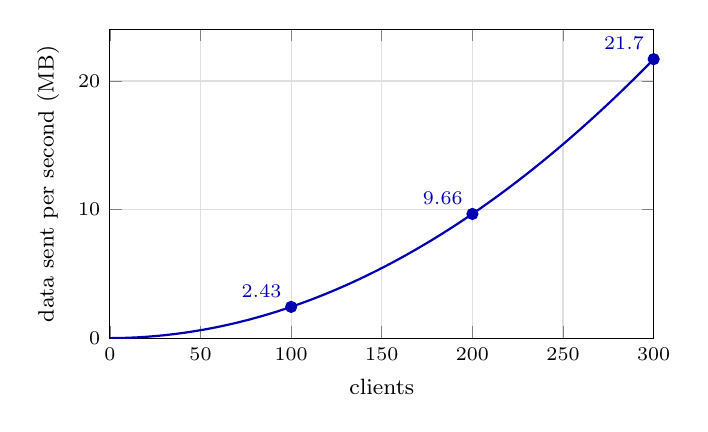
\begin{tikzpicture}
\begin{axis}[width=0.7\textwidth,height=5.5cm,xlabel={clients},ylabel={data sent per second (MB)},
  xmin=0,xmax=300,ymin=0,ymax=24,grid=major,grid style={gray!25},
  tick label style={font=\scriptsize},label style={font=\footnotesize}]
\addplot[blue!70!black,thick,domain=0:300,samples=60]{20*x*(16+12*x)/1000000};
\addplot[only marks,mark=*,mark size=2pt,blue!70!black,nodes near coords,
  every node near coord/.append style={font=\scriptsize,anchor=south east}]
  coordinates {(100,2.43) (200,9.66) (300,21.7)};
\end{axis}
\end{tikzpicture}
\caption{Data the server must send each second as clients are added (calculated
from the packet format; ENet is similar). Tripling the clients from 100 to 300
multiplies the data about nine times.}
\label{fig:growth}
\end{figure}

\subsection{How clients end up responding less (and recovering)}\label{sec:chain}
A client counts as \textit{responding} if it received at least one new snapshot during the
measurement period. While the server keeps up, every client gets a snapshot every
tick. Once the work per tick is too much, snapshots arrive late, get skipped, or
pile up behind each other, and some clients stop receiving any.

\subsection{Threats to validity}
% TODO: write the threats to validity (ping proxy, protocol-level gaps, one cloud zone and machine type, bot clients, one workload, UDP versus ENet client code paths)
TODO: write the threats to validity.

\section{Conclusion}
% [PROPOSAL] Source: the proposal "Conclusion". It restates the setup (built-in ENet dedicated server vs custom C++ UDP server for
%   a Godot game), what the literature established (UDP for real-time gameplay, C++ for low-overhead server work, dedicated-server
%   topology), and the plan. Keep the structure (what was compared, what is known, what was found), but the plan sentence
%   about "five client counts, three repetitions, 240 minutes" must be replaced with the real results and limits.
% [NEW] Aim for one paragraph: what was built, what was measured, the main result with one or two numbers, and the practical advice
%   for a Godot developer (when ENet is enough, when a custom server pays off).
% TODO: finish this (see next line)
TODO.

\begin{thebibliography}{99}
\bibitem{aukstakalnis2024} L. Aukstakalnis, ``Server-client networking implementation using the Godot game engine,'' 2024.
\bibitem{aldhief2018} F. T. Al-Dhief \emph{et al.}, ``Performance comparison between TCP and UDP protocols in different simulation scenarios,'' \emph{Int. J. Eng. Technol.}, vol. 7, no. 4.36, pp. 172--176, 2018.
\bibitem{jones2025} C. Jones, ``Go UDP programming: A beginner-friendly guide to building fast, real-time apps,'' \emph{DEV Community}, Oct. 29, 2025. [Online]. Available: \url{https://dev.to/jones_charles_ad50858dbc0/go-udp-programming-a-beginner-friendly-guide-to-building-fast-real-time-apps-4ik}. Accessed: Feb. 27, 2026.
\bibitem{retunsky2023} E. Retunsky, ``Benchmarking low-level I/O: C, C++, Rust, Golang, Java, Python,'' \emph{Star Gazers}, Mar. 26, 2023. [Online]. Available: \url{https://medium.com/star-gazers/benchmarking-low-level-i-o-c-c-rust-golang-java-python-9a0d505f85f7}
\bibitem{godotdedicated} Godot Foundation, ``Exporting for dedicated servers,'' \emph{Godot Engine Documentation}, 2026. [Online]. Available: \url{https://docs.godotengine.org/en/stable/tutorials/export/exporting_for_dedicated_servers.html}. Accessed: Feb. 27, 2026.
\bibitem{godotudp} Godot Foundation, ``UDPServer,'' \emph{Godot Engine Documentation}, 2026. [Online]. Available: \url{https://docs.godotengine.org/en/4.4/classes/class_udpserver.html}. Accessed: Feb. 27, 2026.
\bibitem{ahde2017} J. Ahde, ``Real-time Unity multiplayer server implementation,'' B.S. thesis, 2017.
\bibitem{arboleda2023} F. J. M. Arboleda, M. R. Arias, and J. A. H. Riveros, ``Performance of parallelism in Python and C++,'' \emph{IAENG Int. J. Comput. Sci.}, vol. 50, no. 2, pp. 1--13, 2023.
\bibitem{celik2024} A. D. \c{C}elik and G. \c{S}e\c{c}inti, ``Network optimizing software solution for multiplayer gaming,'' \emph{ITU J. Wireless Commun. Cybersecurity}, vol. 1, no. 1, pp. 47--56, 2024.
\bibitem{geeksforgeeks2018} GeeksforGeeks, ``UDP server-client implementation in C++,'' Mar. 22, 2018. [Online]. Available: \url{https://www.geeksforgeeks.org/cpp/udp-server-client-implementation-c/}
\bibitem{zehra2020} F. Zehra, M. Javed, D. Khan, and M. Pasha, ``Comparative analysis of C++ and Python in terms of memory and time,'' \emph{Preprints}, 2020, doi: 10.20944/preprints202012.0516.v1.
\bibitem{unityticks} Unity Technologies, ``Ticks and update rates,'' \emph{Netcode for GameObjects 2.5 Manual}. [Online]. Available: \url{https://docs.unity3d.com/Packages/com.unity.netcode.gameobjects@2.5/manual/learn/ticks-and-update-rates.html}
\bibitem{valvesource} Valve Developer Community, ``Source multiplayer networking.'' [Online]. Available: \url{https://developer.valvesoftware.com/wiki/Source_Multiplayer_Networking}
\bibitem{gettys2011} J. Gettys and K. Nichols, ``Bufferbloat: Dark buffers in the Internet,'' \emph{ACM Queue}, vol. 9, no. 11, 2011.
\bibitem{claypool2006} M. Claypool and K. Claypool, ``Latency and player actions in online games,'' \emph{Commun. ACM}, vol. 49, no. 11, pp. 40--45, Nov. 2006.
\bibitem{bernier2001} Y. W. Bernier, ``Latency compensating methods in client/server in-game protocol design and optimization,'' presented at the Game Developers Conf., 2001.
\bibitem{rfc768} J. Postel, ``User datagram protocol,'' IETF, RFC 768, Aug. 1980.
\bibitem{rfc8085} L. Eggert, G. Fairhurst, and G. Shepherd, ``UDP usage guidelines,'' IETF, RFC 8085, Mar. 2017.
\bibitem{enetdocs} ENet, ``ENet: Reliable UDP networking library.'' [Online]. Available: \url{http://enet.bespin.org/} % TODO: add access date, check
\bibitem{godotmultiplayer} Godot Foundation, ``High-level multiplayer,'' \emph{Godot Engine Documentation}, 2026. [Online]. Available: \url{https://docs.godotengine.org/en/stable/tutorials/networking/high_level_multiplayer.html} % TODO: add access date, check
\end{thebibliography}

\end{document}
